\documentclass[11pt]{article}

\usepackage{algorithm}
\usepackage{algorithmicx}
\usepackage{algpseudocode}
\usepackage{mathtools}
\usepackage{sectsty}
\usepackage{graphicx}
\usepackage{amsfonts}
\usepackage{amssymb}
\usepackage[]{amsmath}

% Margins
\topmargin=-0.45in
\evensidemargin=0in
\oddsidemargin=0in
\textwidth=6.5in
\textheight=9.0in
\headsep=0.25in

\title{ECE 598: Trust in Critical Infrastructure Final Project}
\author{Eric Silk}
\date{\today}


\begin{document}
\maketitle
\tableofcontents
\pagebreak

%--Paper--
\section{Introduction}
Renewable energy resources have, in recent years, grown significantly in
popularity. Many are physically distributed as a consequence of their method of
generation. For instance, solar panels are capable of generating power as a
function of their unit area, all else being equal.  Thus, to increase the amount
of power being generated, one must increase the total area of the panel -- or,
more typically, the number of panels.

For this reason, distributed energy resources (or DER's) become less amenable to
conventional centralized control algorithms. This has led to research in
distributed control algorithms. This paper explores:
\begin{itemize}
    \item An algorithmic primitive known as \textit{robust ratio consensus} used
          in some of these control algorithms
    \item A key security/robusntess flaw in this algorithm
    \item A method that has been developed to ameliorate this flaw
    \item Details of the implementaiton of this fix
    \item Potential flaws with this fix for further research
\end{itemize}
\section{(Robust) Ratio Consensus}
We begin by formulating the regime under which these algorithms operate. We
assume DER's are separated in some fashion -- whether logically, physically, or
otherwise -- and are controlled by a governing agent.  These agents are capable
of communicating via some abstract channel that may be directed and lossy (e.g.
TCP/IP, radio, carrier pigeon); the combination of these agents and the
communication channels forms a graph $\mathcal{G} = \{\mathcal{V},
    \mathcal{E}\}$.  So long as this graph is \textit{strongly connected}, we can
proceed with the following algorithm.

Suppose there is some global quantity of interest to be calculated, the equation
for which is:
\begin{equation}
    r^*
    \coloneqq \frac{y_1 + y_2 +\ldots + y_n}{z_1 + z_2 + \ldots + z_n}
    = \frac{\sum_{i\in\mathcal{V}}y_i}{\sum_{i\in\mathcal{V}}z_i}
\end{equation}
where each $y_i$ and $z_i$ is agent $i$'s local quantity.
This is a \textit{ration of sums}, and arises naturally in many engineering
problems (or, perhaps less naturally, the problem can be reformulated to use
this equation). For instance, an unweighted average can be found by setting
$y_i$ to the local quantity and $z_i$ to 1.

While we could use a message-passing protocol to do a sort of state replication
across all agents, this can become unwieldy in large graphs and graphs with a
large diameter. Furthermore, it may be desirable to retain some notion of
privacy and not have your local quantity known. To solve this, we will use the
so-called \textit{ratio consensus} (RC) algorithm which, as its name suggest, allows
disparate agents to come to a consensus about the global ratio $r^*$. In
particular, we will use a variant that is robust to packet drops (recall the
channels may be lossy!) known as the \textit{running sum ratio consensus} (RSRC)
%\cite{robust_rc}.

The algorithm, conducted from the perspective of agent $j$:
\begin{algorithm}
    \caption{Robust Ratio Consensus}
    %\hspace*{\algorithmicindent}
    \textbf{Initialization:}
    \begin{algorithmic}
        \State $x_j[0] \gets [y_j0, z_j0]^T$, $\phi_j[0]\gets[0,0]^T$,
        $\psi_{ji}\gets[0,0]^T$, $\forall v_i\in\mathcal{N}_j^-$
    \end{algorithmic}
    \textbf{Iteration:}
    \begin{algorithmic}
        \For{$k\geq0$}
        \State \textbf{Compute:} $\phi_j[k+1] = \phi_j[k] + \frac{x_j[k]}{D_j^+}$
        \State \textbf{Broadcast:} $\phi_j[k+1]$ to all $v_i\in\mathcal{N}_j^+$
        \State \textbf{Receive:} $\phi_i[k+1]$ from all $v_i\in\mathcal{N}_j^-$
        \State \textbf{Set:} $\psi_{ji}[k+1] = \phi_i[k+1]$ if $\phi_i[k+1]$ arrives; $\psi_{ji}[k]$ otherwise
        \State \textbf{Compute:} $x_j[k+1] = \frac{x_j[k]}{D_j^+} + \sum_{v_i\in\mathcal{N}_j^-}\left(\psi_{ji}[k+1]-\psi_{ji}[k]\right)$
        \State \textbf{Output:} $r_j[k+1] = \frac{y_j[k+1]}{z_j[k+1]}$
        \EndFor
    \end{algorithmic}
\end{algorithm}

The algorithm will converge \textit{asymptotically} to the true global value
$r^*$ as $t\rightarrow\infty$\footnote{We neglect stopping conditions, but in
    short: another algorithm called Max-Min (or Min-Max) Consensus is used to
    determine the maximum and minimum ratio estimate in the graph. If the difference
    between the two falls below some tolerance, we say it's ``good enough'' and move
    on to more interesting things.}.
The robustness to dropped packets comes from the use of the differencing operations. Dropped packets
merely delay convergence somewhat.

There are some additional practical considerations for this algorithm. First, of
course, any consensus algorithm is beset by the spectre  of Byzantine failures.
We posit that, while a theoretical problem for convergence, most modern
communication methods are reliable enough to not be of practical concern (woe to
those who selected carrier pigeons from the suggested communcation channels!).
Second, while this algorithm is distributed and thus almost assuredly
asynchronous, we do need a way of synchronizing. Otherwise, different hardware,
different implementations, or different paths in the program may cause one agent
to complete an iteration and move on well before the others. To resolve this, we
assume each device is capable of knowing the current time to a reasonable degree
of accuracy and precision within a common epoch. This can be managed through
protocols such as NTP or PTP, the use of a GNSS receiver, etc. Then, each round
of the algorithm is bounded via temporal barriers. Any traffic from other agents
from iteration $k-1$ or $k+1$ reaching the local agent during iteration $k$ is
logged and discarded. Finally, there is a maximum number of rounds (or
equivalently overall time) within which the algorithm must converge to prevent a
failure to act in a timely fashion, as well as an alternative action that can be
taken in the event of a failure to converge.

\section{Trust Issues}
While this algorithm seems fairly robust, it is entirely trusting of its
in-neighbors.  Should another agent introduce some error, either due to a benign
bit flip or a malicious manipulation, it will then advertise an incorrect value
to it's out-neighbors. They will, in turn, ingest this erroneous value,
calculate a new (erroneous) local value, and so on.  While it would be bad
enough if the algorithm then failed to converge, a more sinister result occurs:
it converges, but to an incorrect value. I expect i needn't inform the reader of
the dangers of misoperation in critical operations, but one can imagine the
catastrophic effects of a generator exceeding its rated RPM.

How, then, to assess the credibility of those feeding us information? In
personnel security, such as when performing a background investigation, it's
common to require personal or professional references. While it may be possible
for a bad actor to lie about their background, intentions, etc., it is harder to
collude with one or more third parties to sell the decption. We can adopt this
notion to extend the trusting RSRC algorithm into one that adheres to the
Russian proverb: ``Trust, but verify.''

\section{Invariants: Trust...but verify}
To understand the attack model we are interested in, some cases we do not consider include:
\begin{itemize}
    \item The algorithm begins with error; i.e. we do not consider the case
          where an agent's initial values are incorrect, only that during operation
          some error is introduced
    \item The communcation channels themselves are untrustworthy; i.e. we do not
          consider man-in-the-middle (MITM) attacks
    \item The error is introduced after convergence; i.e., the algorithm
          converges but the local value $r_i$ is corrupted later
\end{itemize}
We are solely interested in the case where an error is introduced in some iteration $0<k<k_{final}$.

The communications graph must be extended to allow for a node to hear from it's
in-neighbors' in-neighbors, or it's \textit{two-hop} in-neighbors. Concretely,
this could be achived by a high-power radio broadcast, a separate ``topic'' in a
Pub/Sub scheme, etc.

Then, this ability must be exercised \textit{stochastically}. If it occurred at
every transmission, it would be conceptually identical to these two-hop
neighbors being regular neighbors. If it occurred \textit{periodically}, malicious
actors could inject errors that could ten be undone just before this period expires,
slowing or possibly preventing convergence within a desired time limit. Similarly, they may
be able to take advantage of timing wherein they inject an error in such a way as to
cause convergence to an incorrect value before another check occurs.

Now, both of these attacks are still possible in practice, but remove assurances
that they won't be detected. Instead, an attacker must weigh the risk/cost of
detection vs. the value of a succesful attack.

Unfortuntely, Prof. Alejandro isn't comfortable with me sharing details of his
as-to-yet unpublished algorithm. Instead, I'll provide a rough outline of the
invariant method follows:
\begin{algorithm}
    \caption{Shadow Banning Running Sum Ratio Consensus}
    \textbf{Initialization:}
    \begin{algorithmic}
        \State $x_j[0] \gets [y_j0, z_j0]^T$, $\phi_j[0]\gets[0,0]^T$,
        $\psi_{ji}\gets[0,0]^T$, $\forall v_i\in\mathcal{N}_j^-$
        \Comment The familiar RSRC Quantities
        \State $\mu_{il}^{(j)}[0] = [0,0]^T \forall v_i\in\mathcal{N}_j^-$, $\forall l\in \mathcal{N}_i^-$
        \Comment Like $\psi$, but for the two-hop neighbors
        \State $\mathcal{T}_j[0] = \mathcal{N}_j^-$, $\Delta\mathcal{T}_j[0] = \emptyset$
        \Comment Our set of trusted and untrusted in-neighbors, respectively
        \State $\mathcal{T}_i^{(j)}[0] = \mathcal{N}_i^-\forall i\in\mathcal{N}_j^-$
        \Comment Our in-neighbors trusted in-neighbors
    \end{algorithmic}
\end{algorithm}
Iteration proceeds much the same as RSRC, with a few primary modifications:
\begin{itemize}
    \item Broadcasts occur either to our out-neighbors with probabilty $1-p_j$,
          or to our out-neighbors \textit{and} their out-neighbors with probability
          $p_j$.
    \item Broadcasts include both $\phi_j[k+1]$ and our newly untrusted nodes
          $\mathcal{T}_j[k] \backslash \mathcal{T}_j[k+1]$
    \item Receive from our one-hop and (possibly) our two-hop neighbors
    \item Track which two-hop neighbors we hear from
    \item If we hear from \textit{all} of an in-neighbor's in-neighbors,
          calculate an invariant quantity $\gamma_{i}^{(j)}$ using knowledge of
          it's out-degree, the transmissions it sent to us ($\phi_i$), and the values that
          were sent to it ($\psi_{il}$).
    \item If this quantity $\gamma_{i}^{(j)}$ is nonzero (or not close enough to
          zero in finite precision), mark it as untrustworthy and remove it from our
          trusted set.
    \item Calculate our new quantity $x_j[k+1]$ without the use of this node's
          contributions and incorporating the two-hop contributions when available in
          its stead
\end{itemize}

\section{Implementing the Invariant Method}
\subsection*{Prior Work}
The aforementioned RSRC algorithm has been implemented in a C++ library along with all the necesscary
infrastructure to enable demonstrations -- basic task scheduling and management,
communications, packet routing, etc.

\medskip
\noindent
But...

\medskip
\noindent
\noindent
Development in this environment is...slow. While the RSRC task was written to be flexible enough to
build upon (use unique per-task packets, set the quantity and type of num/den
values, etc.), the algorithm described above was different enough to warrant a
rewrite. At least, until I could wrap my head around it conceptually.
Unfortunatley, C++ is a harsh mistress\footnote{I'm also an extremely mediocre
    C++ programmer. I miss having senior software engineers I could ask dumb
    questions...}. After several days of weird CMake complaints, obnoxious
compilation errors, and slow build times I decided to cast it aside and rebuild
a prototype algorithm in Python.

\subsection*{Python Implementation}
This implementation attempted to adhere to the notation used in the paper as
closely as possible. It is synchronous, and relies on a wrapper to call each
agent manually. This is fine for demo/experimental purposes, as the same effect
in an asynchronous implementation is achieved through the use of time gating.
The only detail of note about this is that there are two sections of each
iteration: the broadcast, and then the reception/update.  Each agent's broadcast
method is called, and then each agent's reception/update method is called.
Like the C++ implementation, I have elected to use ZMQ for messaging.

\subsubsection*{The Numerical Experiments}
The experimental setup consists of 5 nodes (agents 1-5) connected as seen in
Fig. \ref{fig:graph} (note that self-loops are included for clarity). A simple
distributed averaging problem is attempted, with each agent taking it's own ID as the local value; so:
\[ r^* = \frac{1 + 2 + 3 + 4 + 5}{1 + 1 + 1 + 1 + 1} = 3 \]

In the first experiment, we will verify nominal operation. In the next, we will introduce
an error into a node at some iteraion $k>0$; in particular, agent 3 will have 2000 added to its numerator
and 3000 to its denominator. If the algorithm works correctly, we may see some perturbation
at this time, but it should then begin to reconverged to 3 (the fact that the
average will remain the same when agent 3 is removed was not intentional, but as
we will see, proved immaterial).

\begin{figure}
    \centering
    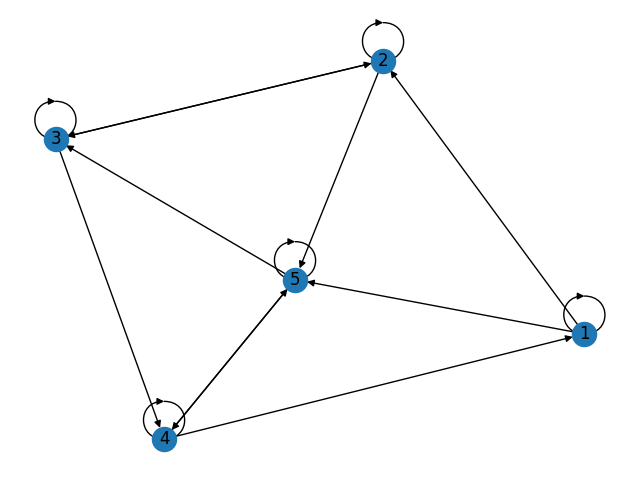
\includegraphics[width=0.5\textwidth]{img/graph.png}
    \caption{The experimental communciations graph}
    \label{fig:graph}
\end{figure}

\subsubsection*{What's working}
The reimplemented algorithm functions correctly when there is no error introduced (Fig. \ref{fig:central_good}).
\begin{figure}[h!]
    \centering
    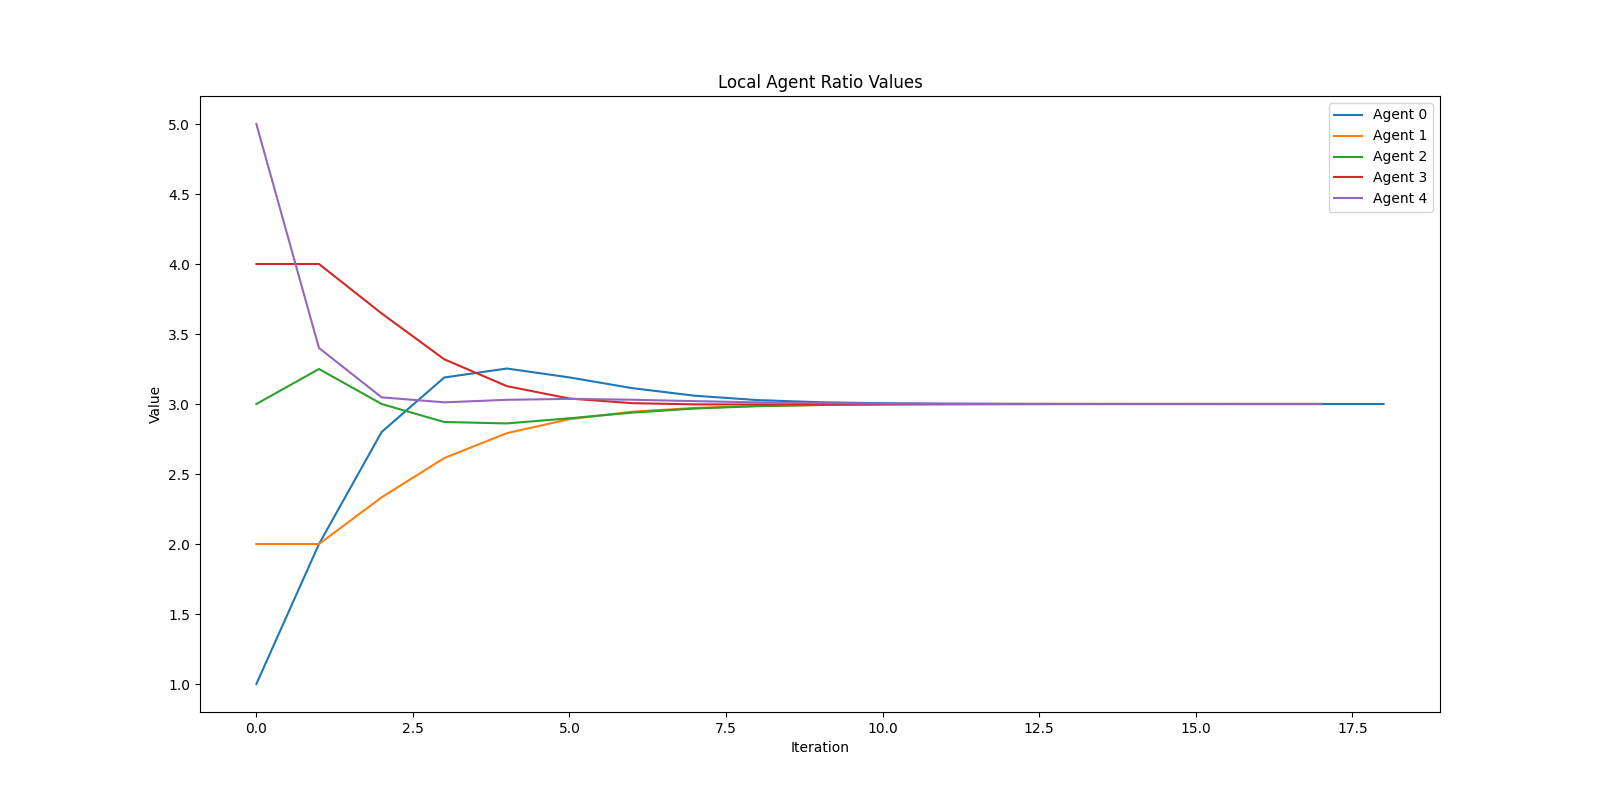
\includegraphics[width=\textwidth]{img/vanilla_centralized_ratios.png}
    \caption{Agent's knowlede of their local ratio (Global ratio: 3)}
    \label{fig:central_good}
\end{figure}
In addition, we can see that $\gamma_i^{(j)}$ stays at $\approx0$ for all nodes
(Figs. \ref{fig:gg0}, \ref{fig:gg1}, \ref{fig:gg2}, \ref{fig:gg3}, \ref{fig:gg4}).
\begin{figure}[h!]
    \centering
    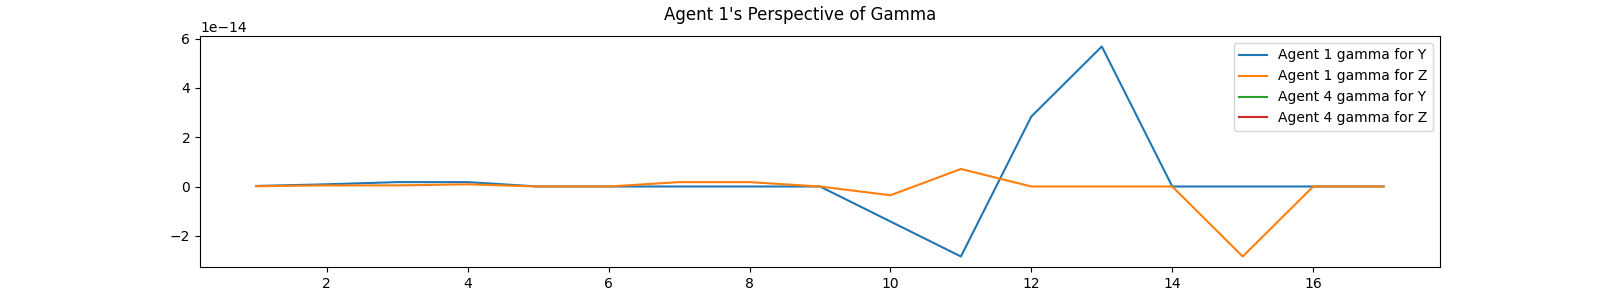
\includegraphics[width=\textwidth]{img/vanilla_agent_0_gammas.png}
    \caption{Agent 1's calculated $\gamma$ for it's in-neighbors}
    \label{fig:gg0}

    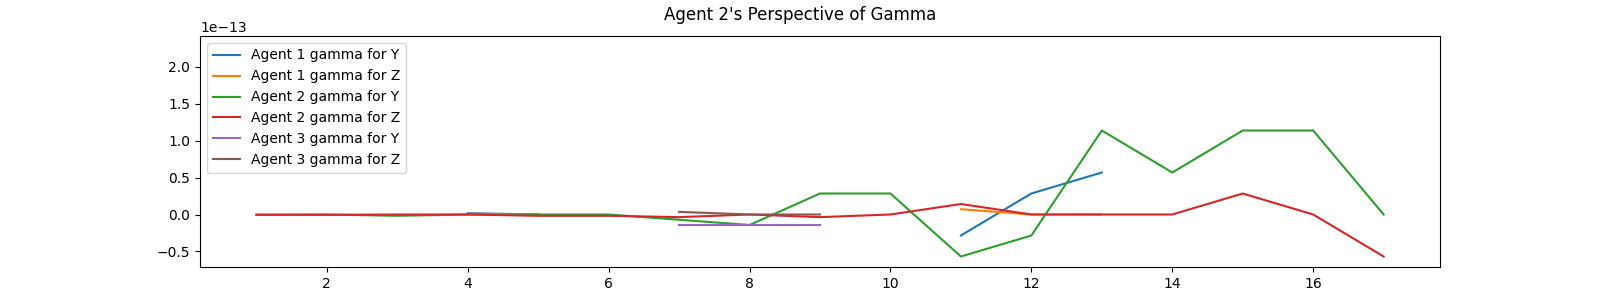
\includegraphics[width=\textwidth]{img/vanilla_agent_1_gammas.png}
    \caption{Agent 2's calculated $\gamma$ for it's in-neighbors}
    \label{fig:gg1}

    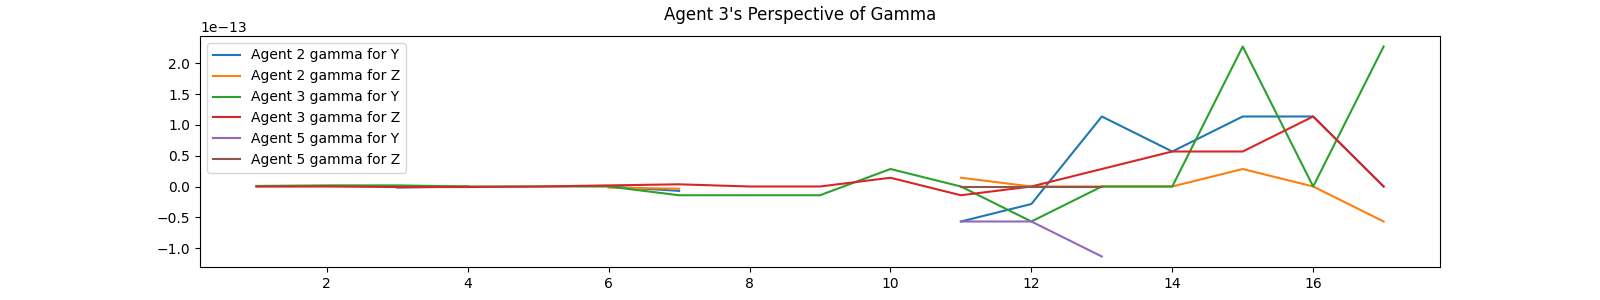
\includegraphics[width=\textwidth]{img/vanilla_agent_2_gammas.png}
    \caption{Agent 3's calculated $\gamma$ for it's in-neighbors}
    \label{fig:gg2}

    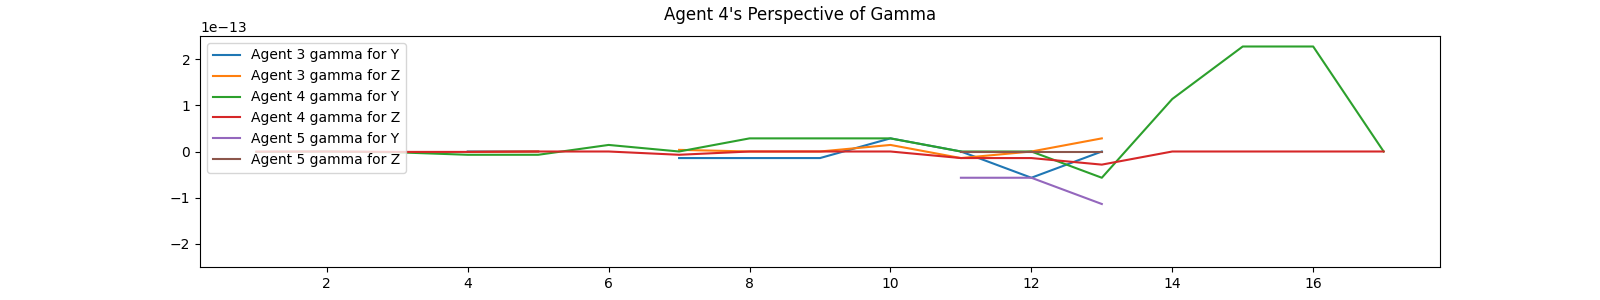
\includegraphics[width=\textwidth]{img/vanilla_agent_3_gammas.png}
    \caption{Agent 4's calculated $\gamma$ for it's in-neighbors}
    \label{fig:gg3}

    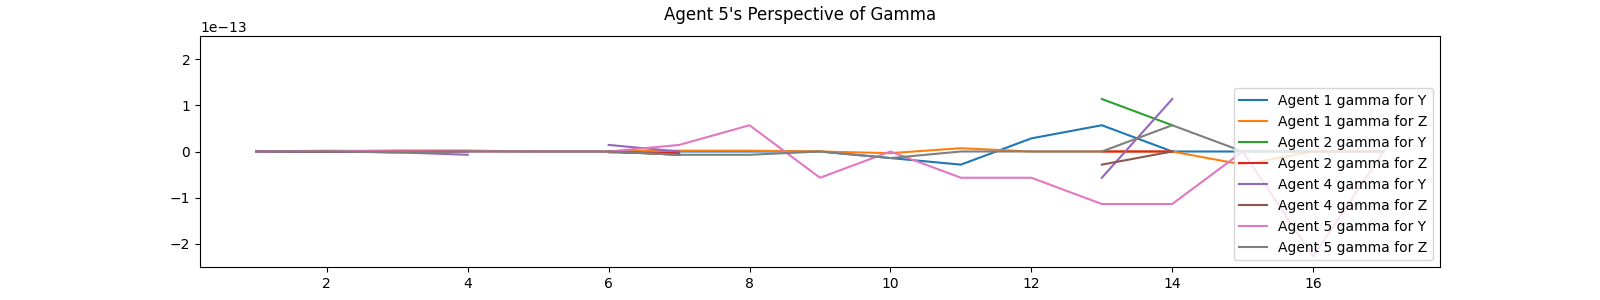
\includegraphics[width=\textwidth]{img/vanilla_agent_4_gammas.png}
    \caption{Agent 5's calculated $\gamma$ for it's in-neighbors}
    \label{fig:gg4}
\end{figure}
So far, so good!

In addition, when an error is injected into one node (here, Agent 3 on iteration $k=3$),
we can see that gamma for the nodes tracking it does become non-zero
(Figs. \ref{fig:bg0}, \ref{fig:bg1}, \ref{fig:bg2}, \ref{fig:bg3}, \ref{fig:bg4})
and it is removed from the trusted set (note the truncation of the data).
\begin{figure}[h!]
    \centering
    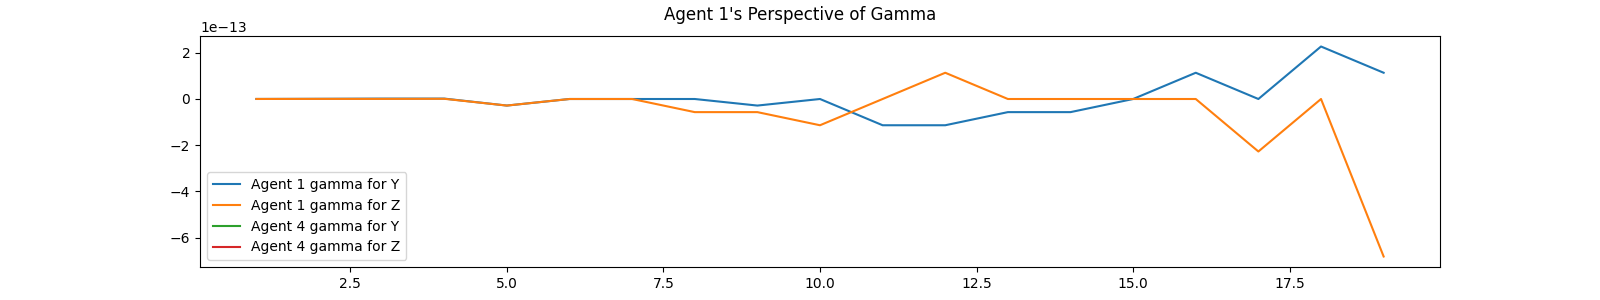
\includegraphics[width=\textwidth]{img/error_agent_0_gammas.png}
    \caption{Agent 1's calculated $\gamma$ for it's in-neighbors}
    \label{fig:bg0}

    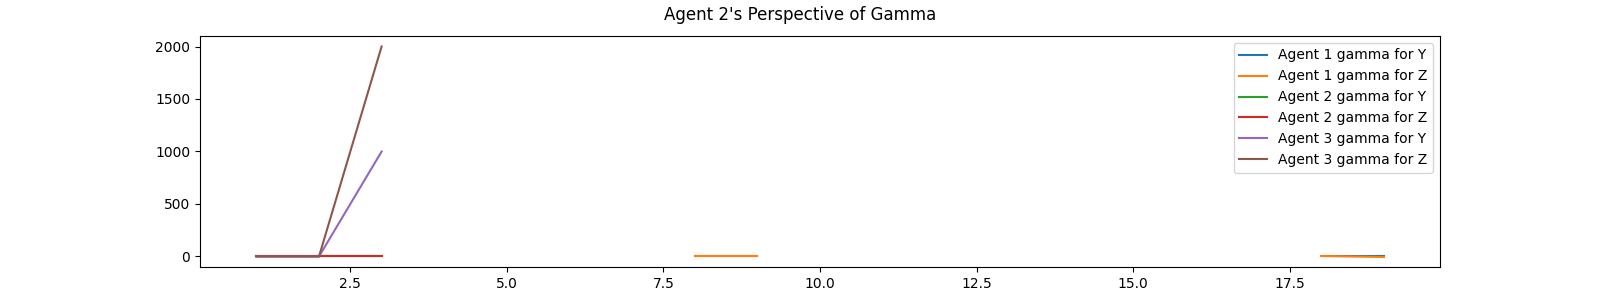
\includegraphics[width=\textwidth]{img/error_agent_1_gammas.png}
    \caption{Agent 2's calculated $\gamma$ for it's in-neighbors}
    \label{fig:bg1}

    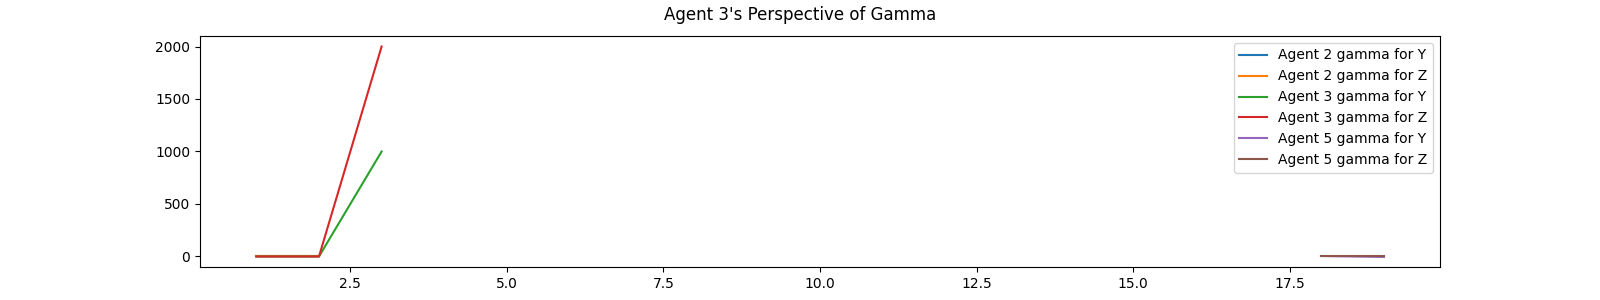
\includegraphics[width=\textwidth]{img/error_agent_2_gammas.png}
    \caption{Agent 3's calculated $\gamma$ for it's in-neighbors}
    \label{fig:bg2}

    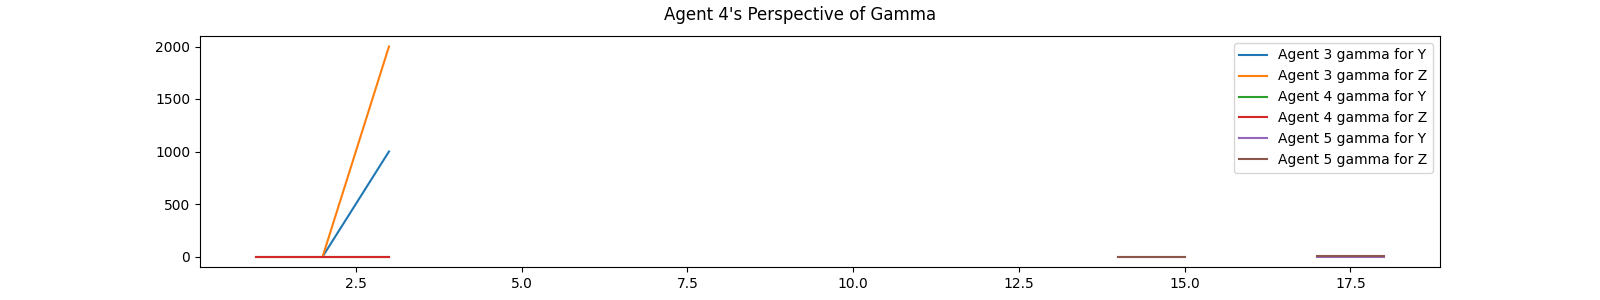
\includegraphics[width=\textwidth]{img/error_agent_3_gammas.png}
    \caption{Agent 4's calculated $\gamma$ for it's in-neighbors}
    \label{fig:bg3}

    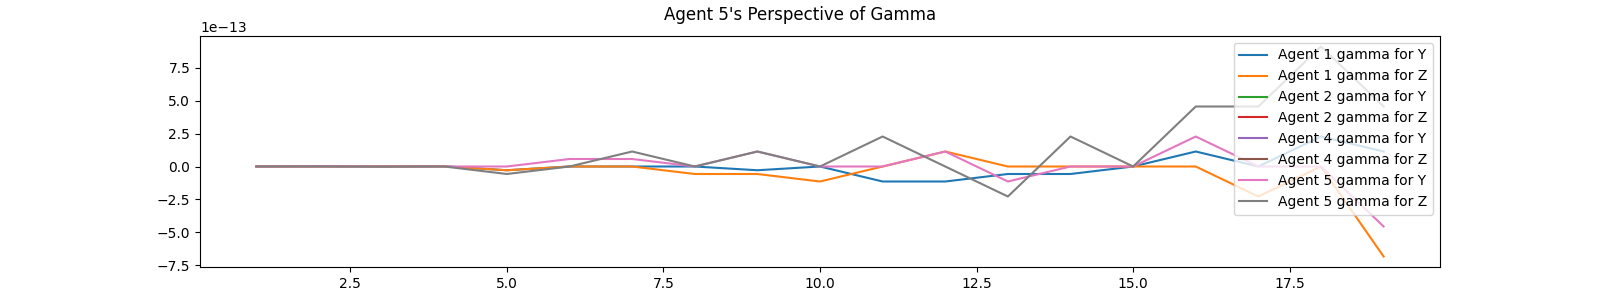
\includegraphics[width=\textwidth]{img/error_agent_4_gammas.png}
    \caption{Agent 5's calculated $\gamma$ for it's in-neighbors}
    \label{fig:bg4}
\end{figure}

\subsubsection*{What's \textit{not} working}
It wouldn't be a final project being written up 8 hours before it's due without some
caveats. During implementation, there appeared to be a typo in the algorithm.
After seeking clarification with Prof. Alejandro, he confirmed that yes, in fact,
we were required to calculate the value of $x$ on another node, using the
fact we know it's out-degree and backing that value out from what it sent. Fair enough.

Unfortunately, it required time travel. To clarify, on iteration $k$ we
calculate  $\phi_j[k+1]$ based on our local copy of $x_j[k]$, and receive
$\phi_i[k+1]$ from in-neighbors. We then calculate $x_j[k+1]$ based on all of
these received $\phi_i[k+1]$s.  This \textit{also} allows us to back out
$x_i[k]$. The trust calculation, as it was originally written, required
$x_i[k+1]$ at iteration $k$, meaning we would need to to receive $\phi_i[k+2]$.
As I understand it, time isn't linear, but it is monotic. Alas.

But fear not! It was decided that it was valid to \textit{lag} our trust
verification by one iteration -- that is, we can't determine if in an iteration
we are being lied to, but \textit{can} determine it on the next iteration! And,
as demonstrated by the simulations, the detection still works; \textit{however},
removal of the agent isn't working quite as planned. It is unclear to me if it
is an error in implementation, a failure to adjust some of the iteration indices
used in the algorithmic listing I am working off of, or a failure to properly
remove the  \textit{historical} influence of said agent.

\begin{figure}[h!]
    \centering
    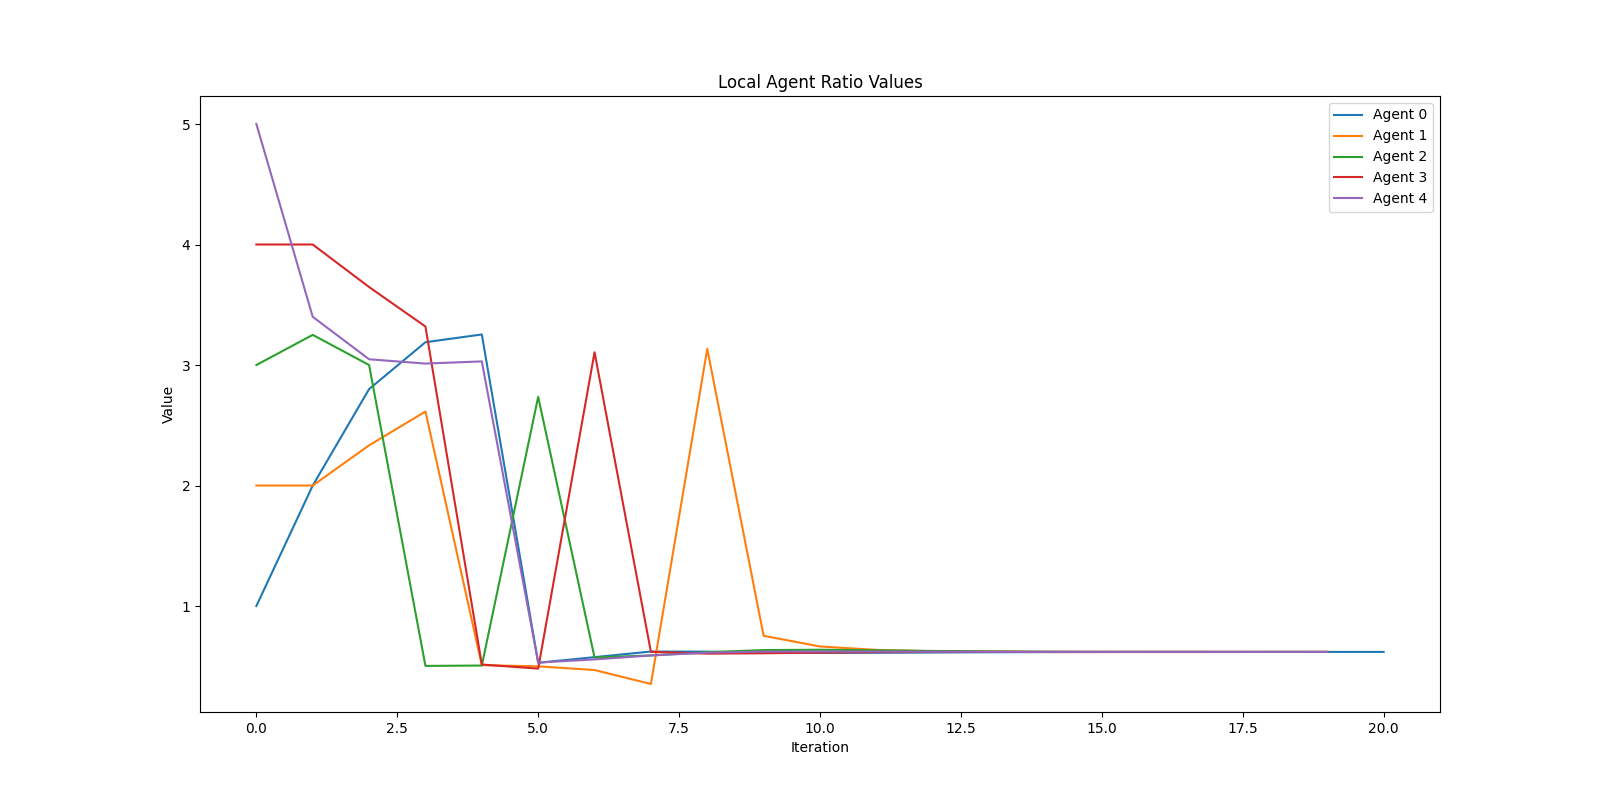
\includegraphics[width=\textwidth]{img/error_centralized_ratios.png}
    \caption{Agent's knowlede of their local ratio, with a grevious error
        committed by Agent 3 on iteration 3}
    \label{fig:central_bad}
\end{figure}

This is visible in Fig. \ref{fig:central_bad}, where we can see the trajectories
suddenly shift quite dramatically and, instead of converging on 3, end on around
0.75.

\subsubsection*{TODO}
Obviously, next steps are to figure out what is causing this error and correct
it to verify empiraclly that this algorithm works. Then, we can run some basic
studies on attacks discussed in the next section, and implement an asynchronous
version of it to run in the existing C++ library (preferably with more
intelligent data strutures, variable names, etc.) and repeat the same
experiments for validation.

\section{Attacking the Invariant Method}
So now we have a method\footnote{...sort of. See "What's not working" for details} for detecting a certain class of errors/attacks,
enabling perfect operation of our code-base, serious profits to be had from
selling this wonderous tech, our favorite sports team winning, and peace in the
Middle East. Right?

\subsection*{Shadow Banned but Still There}
A key feature adverstised in this algorithm is that the offending agent(s) can
be removed without their knowledge. The perceived benefit is that, if the node
is malicious, it would then be unable to take remedial action in an attempt to
continue to wreak havoc.

However, if the error introduced is \textit{not} an attack, the agent will
continue to operate in ignorance and potentially converge to an incorrect value
-- \textbf{which it may then still act upon}.

\subsection*{Constraints on Topology}
Suppose there is one or more nodes in a graph such that their removal
would violate the assumption that $\mathcal{G}$ is strongly connected.
We can call these ``keystone'' nodes. The use of this method would then
create a vulnerability in which an attacker intentionally introduces
error on such a node to cause it to be declared untrustworthy and removed.

I can imagine two possiblities. In one, the graph stays connected via the
two-hop edges, allowing the asymptotic convergence property to be preserved but
slowing the rate of convergence to such a degree that it prevents finite-time
convergence within an allowable window. In the other (and I would need to spend
some time to determine if this is actually possible...), the two-hop connections
are still insufficient to have a strongly connected graph, preventing
even asymptotic convergence.

\subsection*{A Friend of a Friend}
Although addressed in the paper, the fact  that the use of two-hop neighbors
only insulates you from non-adjacent faulty agents is somewhat understated. As
soon as two are adjacent, this falls apart. It is mentioned that this can be
corrected by increasing the broadcast to include \textit{three-hop} neighbors,
and so on.

Unfortunately, in small graphs, this quickly exhausts the pool of available
agents.  One possible conclusion is that, for this method, larger systems become
more secure.  It would be interesting to explore the tradeoffs in attack
surface, convergence time, etc.  vs. the improved probabilty of detecting n-hop
errors.  Of course, this will do nothing to help systems that are intentionally
small, such as microgrids, which may quickly decide that they're better of just
using state replication and centralized algorithms.

\subsection*{Playing the Lottery}
A key weakness of this method is that it is intentionally stochastic. The
theoretic guarantees about convergence and detection are predicated on the
characteristic of \textit{asymptotic convergence}; that is, no finite time
stopping. Yes, if you have a non-zero probabilty of something happening, and
allow a system infinite time, it will eventually happen.

This goes away as soon as we introduce a finite-time stopping condition.
The probabilty of a detection occuring then becomes a function of the
two-hop transmission probabilty (and probabilty of a packet drop) \textit{and}
the time between an error/attack until convergence. In practice, on small graphs
(such as what might be found in a microgrid), we see convergence occurring in
relatively few iterations ($<20$ in the numerical experiment).

This quickly shifts the discussion from the cozy world of theoretic guarantees
and ``almost surely'' into a discussion of likelihoods, cost vs. benefits, etc.
This isn't inherently a problem -- indeed, it could be argued that nearly all of
security boils down to this exact dilemma. However, industrial and government
practice often tends either towards hamstringing via over-cautious risk aversion or
decapitation from over-zealous risk tolerance.

Analysis, either analytically or empircally, of a system in question quickly
becomes a must to inform architects of desirable topologies and n-hop
probabilties, increasing the complexity and possibly stifling adoption.

\subsection*{A Witch Hunt}
Another issue with this is that it shifts the trust from the ratio consensus algorithm
to the broadcast of the ``untrusted'' nodes. It isn't entirely clear to me yet
how this will handle a malignant node falsely declaring one of it's in-neighbors to be
erroneous. A naive implementation (\textit{cough} certainly not mine \textit{cough})
would immediately cease contact with said node. A more refined approach
would be to take this broadcast under advisement, and require multiple
nodes to make this declaration before accepting it. Or perhaps it can be
rendered un-needed, where each node makes its own determinations
solely based upon these two-hop broadcasts and no broadcast of trust need occur.

\subsection*{An $\epsilon$ Problem}
Finally (I think...), the analytic guarantees of the algorithm exist within the
realm of infinite precision. Computer systems have no such luxury, introducing a
need for tolerances when assessing the invariant.  This, in turn, introduces a
receiver operating characteristic (ROC) for detecting malicious agents, a need to
set an acceptable false positive/false negative rate, and so on.

The complexity of that aside, it could also enable degradation of the algorithm
by ``flying under the radar'' and introducing errors small enough to escape
detection, while still producing subtly incorrect results.


\end{document}